\chapter{Analysis}

\section{Requirements}

In this section, the requirements of the project are presented.

\subsection{Functional Requirements}

The functional requirements of the project are described in this subsection.

\subsection{Non-Functional Requirements}

The non-functional requirements of the project are described in this subsection.

\subsection{Constraints/Other Requirements}

Any constraints or other requirements on the project are described in this subsection.

\section{Actors}

The actors who can interact with the web console system consist of the following:
\begin{itemize}
    \item \textbf{User:} The user is the actor who can browse the system to view running and completed experiments and their results.
    \item \textbf{Admin:} The admin is the actor who can manage the system, including creating and deleting configurations and experiments, and viewing the results of experiments.
\end{itemize}

\section{Use Case Modeling}

\subsection{Use Case Diagram}

\begin{figure}[ht!]
    \centering
    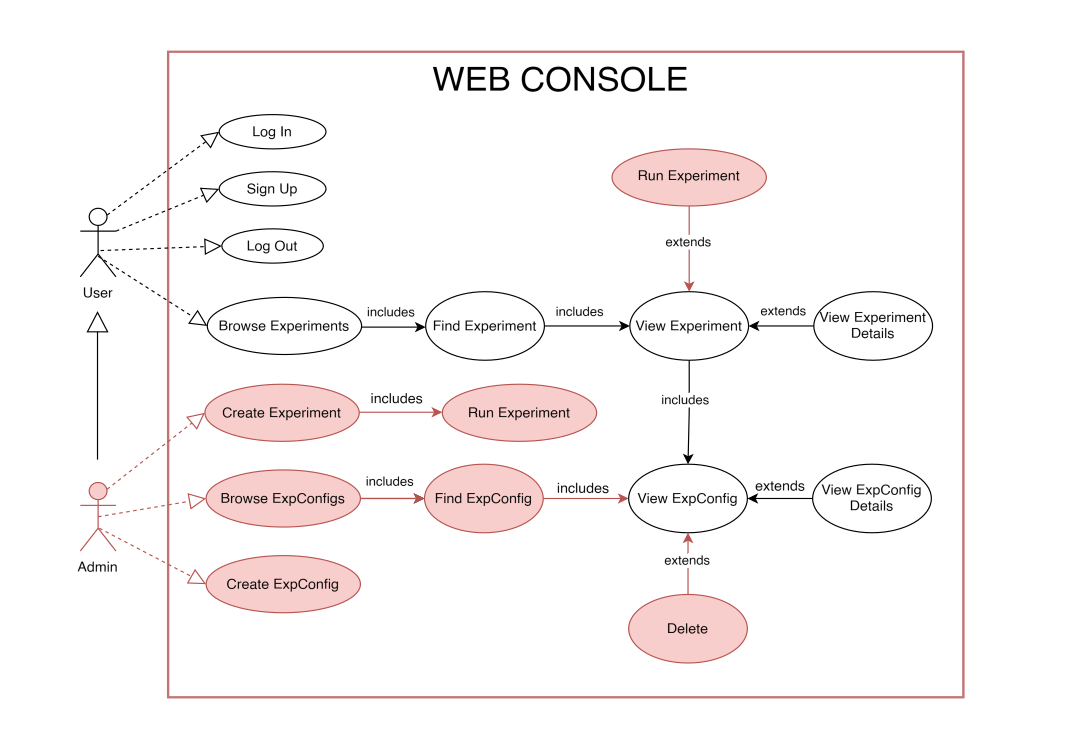
\includegraphics[width=0.8\textwidth]{images/2_analisys/FL_class_diag.drawio.png}
    \caption{Use Case Diagram}
    \label{fig:use_case_diagram}
\end{figure}

\subsection{Scenarios}

\begin{table}[ht!]
    \centering
    \caption{Use Case: Find Recipes}
    \begin{tabular}{|Sl|Sl|}
        \hline
        \textbf{\textit{Use Case}}      & \textbf{Find Recipes}                                     \\ \hline
        \textbf{Primary Actor}           & User                                            \\ \hline
        \textbf{Secondary Actor}         & -                                               \\ \hline
        \textbf{Description}             & Allows the user to find a specific recipe       \\ \hline
        \textbf{Pre-Conditions}          & User must be logged in                          \\ \hline
        \textbf{Main event steps}        & 1. The user navigates to the “Search” feature   \\ 
                                          & 2. The user enters a string                     \\
                                          & 3. The system searches the recipe database for  \\ 
                                          & matching results (title, keywords, description) \\ 
                                          & 4. Upon finding matching posts, the system      \\ 
                                          & displays the search results                     \\ \hline
        \textbf{Post-Conditions}         & The user views a list of recipes matching the   \\ 
                                          & search criteria if there are any                \\ \hline
        \textbf{Correlated Use cases}    & View Recipe, Browse Recipes                     \\ \hline
        \textbf{Alternative event steps} & -                                               \\ \hline
    \end{tabular}
\end{table}
\subsection{Analysis Class Diagram}

The analysis class diagram of the project is presented in this subsection.

\subsection{Sequence Diagrams}

The sequence diagrams of the project are presented in this subsection.

